\chapter{Dimensionering af fundament}

Metatekst
\section{Fundering}
Et fundament er en del af et bygværk, hvor formålet er at overføre belastningen fra bygningen til underliggende, bærende jordlag. Der findes mange forskellige funderingsmetoder, for eksempel pælefundering og direkte fundering, og kan i nogle tilfælde kombineres. De to mest almindelige funderingsmetoder er pæle- og direkte fundering, hvilke vil blive omtalt i denne rapport.
\newline \indent{     }  Ved direkte fundering støbes fundamentet direkte på terrænet, hvor de bæredygtige jordlag findes relativt tæt under bygningen. Belastningen overføres fra bygningen til jorden igennem vandrette flader. Belastningen på fundamentfladen udgøres af fundamentets egenvægt og bygingens belastning. Hvis belastningen virker på en lang fundamentflade med konstant bredde, er der tale om et stribefundament, der som regel bruges ved fundering af bærende vægge. Modsætningen hertil er punktfundamenter, som er rektangulære eller kvadratiske, og disse bruges for eksempel ved fundering af master, søjler og skorstene \citep[ s. 221]{geoteknik}. Stribefundamentet og punktfundamentet er illustreret på Figur \ref{fig:fundament}. 

\begin{figure}[htbp] \centering
	\begin{minipage}[b]{0.48\textwidth}\centering
		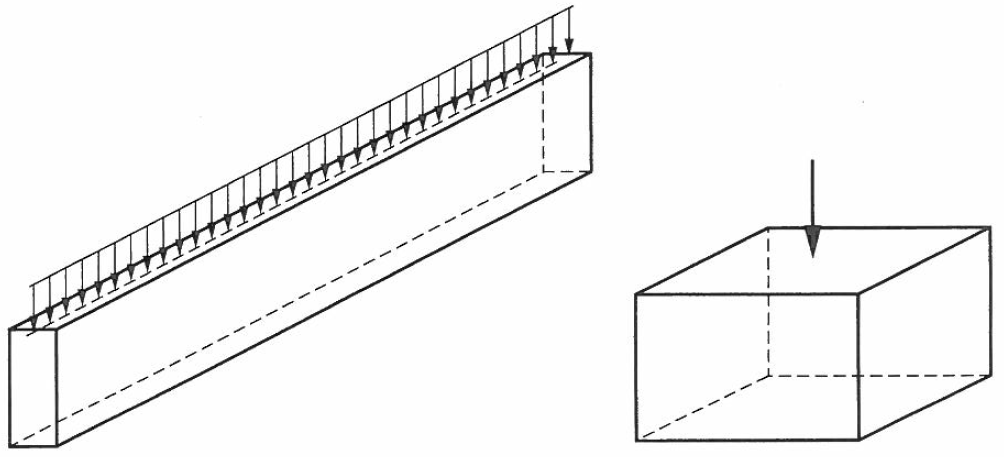
\includegraphics[width=1.0\textwidth]{billeder/fundament.png}
		\caption{Stribefundament og punktfundament \citep[ s. 221]{geoteknik}}
		\label{fig:fundament}
	\end{minipage}\hfill
\end{figure}

\indent{     }  Hvis de bæredygtige jordlag ligger mere end 4-5 meter under bygingen, anvendes ofte pælefundering. Ved pælefundering er søjleformede pæle af træ, beton, og/eller stål, rammet, presset, vibreret eller udstøbt i jorden. Pæleformen er normalt cylindrisk med cirkulært eller kvadratisk tværsnit. Pælefundering benyttes blandt andet når de bærende jordlag ligger så dybt, at direkte fundering vil blive uøkonomisk \citep[ s. 355]{geoteknik}.
\newline
\newline
Valg af funderingsmetode for tilbygningen til Strøybergs Palæ afhænger af jordbunds- og grundvandsforhold samt de belastninger, som konstruktionen er udsat for \citep[ s. 355]{geoteknik}. Det er derfor nødvendigt at have kendskab til områdets geologi omkring Strøybergs Palæ, og at tolke på de boreprofiler, der bliver udført på stedet, hvilket vil gøres i forsøgene i Afsnit 8.4. 

\section{Antagelser}
Idét Aalborg er funderet på meget blødt ler, benyttes boreprofiler fra Hals/Hou, og det antages, at disse boreprofiler er fra området ved Strøybergs Palæ. 
\newline \indent{     }  Forsøgene er udført på baskarpsand fra Sverige, hvilket antages at være sandet fra boreprofilerne.

\section{Forsøg}
For at bestemme styrkeparametre for jorden udføres laboratorieforsøg, der bruges ved dimensionering af fundamentet.
\newline
\newline
Formålet med forsøgene er at bestemme friktionsvinklen, givet ved: 

\begin{center}
	$\varphi = 30^\circ - \frac{3}{U} + (14 - \frac{4}{U}) I_D$
\end{center}

\begin{itemize}
	\item[-] U: Uensformighedtal
	\item[-] $I_D$: Relativ lejringstæthed
\end{itemize}

Friktionsvinklen $\varphi$ er et mål for jords styrke, og skønnes ud fra sigteanalyse samt løs og fast lejring. Ved hjælp af nedenstående fire forsøg bestemmes friktionsvinklen, idét uensformighedstallet og den relative lejringstæthed bestemmes herudfra: 
\begin{enumerate}
	\item Vandindhold
	\item Sigteanalyse
	\item Kornvægtfylde
	\item Løs og fast lejring
\end{enumerate}
Tabeller over resultater, fremgangsmåde, apparaturliste samt fejlkilder for de enkelte forsøg findes i bilag A-D.

\subsection{Forsøg 1: Vandindhold}
Formålet med forsøget er at finde vandindholdet \textit{w} i jordprøven. Vandindholdet er defineret som jordens vægttab i \% af tørvægten ved tørring i et varmeskab ved en temperatur på 105$^{\circ}$C. For naturligt forekommende jordarter kan vandindholdet ligge mellem nul og flere hundrede procent.
\newline
\newline
Vandindholdet beregnes ved:

\begin{center}
	$w = \frac{W_w}{W_s}\cdot 100\% = \frac{(W+sk)-(W_s+sk)}{(W_s+sk)-sk}\cdot 100\%$
\end{center}

\begin{itemize}
	\item[-] $W_w$: Vægten af vandet i prøven [g]
	\item[-] $W_s$: Vægten af det tørrede materiale [g]
	\item[-] W: Vægten af prøven før tørring [g]
	\item[-] sk: Vægten af skålen [g]
\end{itemize}

Forsøget er udført to gange. De fundne værdier for de to udførte forsøg ses i Tabel \ref{tab:bilaga1} i Bilag A. Vandindholdet for de to forsøg er beregnet til:

\begin{center}
	Forsøg 1: $w = \frac{81,\!02 g - 80,\!99 g}{80,\!99 g - 3,\!07 g}\cdot 100\% = 0,\!04\%$
\end{center}

\begin{center}
	Forsøg 2: $w = \frac{89,\!83 g - 89,\!79}{89,\!79 g - 3,\!11 g}\cdot 100\% = 0,\!05\%$
\end{center}

Ud fra de opnåede resultater, kan det konkluderes, at det benyttede materiale vurderes at være tørt og det meget lille vandindhold har ikke indflydelse på de øvrige resultater.
\newline \indent{     }  Til videre beregninger benyttes gennemsnittet for vandindholdet for forsøg 1 og forsøg 2, som er $0,\!04$\%. Dette skal bruges som et rent tal, som er $0,\!0004$. 

\subsection{Forsøg 2: Sigteanalyse}
Formålet med forsøget er at bestemme jordkornenes vægtmæssige fordeling efter størrelse i sand- og grusfraktion, for at beregne uensformighedstallet \textit{U} for jorden:

\begin{center}
	$U = \frac{d_{60}}{d_{10}}$
\end{center}

\begin{itemize}
	\item[-] $d_{60}$: 60\%-fraktilen
	\item[-] $d_{10}$: 10\%-fraktilen
\end{itemize}

Uensformighedstallet fortæller, hvor velsorteret jorden er:

\begin{itemize}
	\item[-] Velsorteret: $U < 2$
	\item[-] Sorteret: $2 < U < 3,\!5$
	\item[-] Ringe sorteret: $3,\!5 < U < 7$
	\item[-] Usorteret: $U > 7$
\end{itemize}

Forsøget er udført to gange, og der er derfor lavet en sigtekurve for hvert forsøg, og uensformighedstallet er udregnet for begge forsøg. 
\newline \indent{     }  Det procentvise gennemfald i hver sigte er beregnet, og herudfra fås sigtekurverne vist på Figur \ref{fig:sigtekurve1} og Figur \ref{fig:sigtekurve2}. Værdierne der er brugt til at finde det procentvise gennemfald på Figur \ref{fig:forsoget} og Figur \ref{forsogto} i Bilag B. 

\begin{figure}[htbp]
		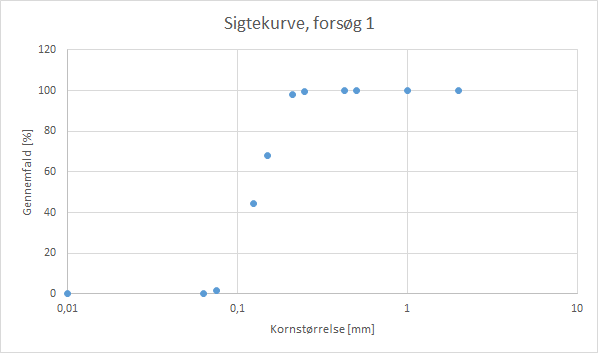
\includegraphics[width=1.0\textwidth]{billeder/sigtekurve1.png}
		\caption{Sigtekurve til forsøg 1}
		\label{fig:sigtekurve1}
\end{figure}

\begin{figure}[htbp]
		\centering
		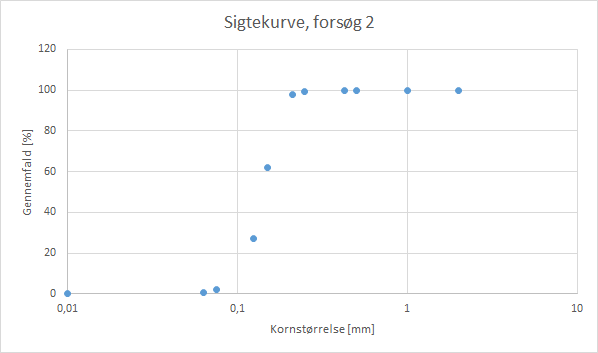
\includegraphics[width=1.0\textwidth]{billeder/sigtekurve2.png}
		\caption{Sigtekurve til forsøg 2}
		\label{fig:sigtekurve2}
\end{figure}

Uensformighedstallet for begge forsøg er beregnet, ved at lave lineær regression imellem henholdsvis 10\% og 60\% og derved finde 10\%-fraktilen og 60\%-fraktilen.
\newline
\newline
Ved det første udførte forsøg er 10\%-fraktilen fundet ved at lave lineær regression imellem sigte med maskestørrelse $0,\!075$ mm og $0,\!125$ mm, hvor følgende ligning fremgår: 

\begin{center}
	$y = 862,\!42x - 63,\!223$
\end{center}

For at finde 60\%-fraktilen er der lavet lineær regression imellem sigte med maskestørrelse $0,\!125$ mm og $0,\!15$ mm, hvor følgende ligning fremgår:

\begin{center}
	$d_{60}=937,\!12x - 72,\!56mm$
\end{center}

Ved forsøg 1 er 10\%-fraktilen og 60\%-fraktilen hermed beregnet til: 
\begin{center}
	$d_{10} = 0,\!08$ og $d_{60} = 0,\!14mm$
\end{center} 

Uensformighedstallet i forsøg 1 er derved:
\begin{center}
	$U = \frac{0,\!14}{0,\!08} = 1,\!67$
\end{center}

Ved forsøg 2 er 10\%-fraktilen, 60\%-fraktilen og uensformighedstallet beregnet til:
\begin{center}
	$d_{10} = 0,\!91$ og $d_{60} = 0,\!15$ og $U = \frac{0,\!15}{0,\!91} = 1,\!64$
\end{center} 
Uddybbende beregninger er vist i Bilag B.

Til videre beregninger benyttes gennemsnittet af uensformighedstallet for forsøg 1 og forsøg 2, som er $1,\!65$. Dette tal fortæller, at jorden er velsorteret, idet $U<2$. Dette stemmer godt overens med de observationer der forinden forsøget var gjort af sandet, hvor blev vurderet til at være ens- og afrundede korn. 

\subsection{Forsøg 3: Kornvægtfylde}
Formålet med forsøget er at finde den relative densitet $d_s$, også kaldet kornvægtfylden, for jordprøven. For jordarter uden organisk indhold kan kornvægtfylden variere fra $2,\!65$ for rent kvartsand til $2,\!85$ for visse lermineraler. I dette forsøg søges altså et resultat der ligger så tæt på $2,\!65$ som muligt.
\newline
\newline
Kornvægtfylden beregnes ved:

\begin{center}
	$d_s = \frac{W_s \rho_w^t}{(W_s + W_2 - W_1)\rho_w^{4^{\circ}}}$
\end{center}

\begin{itemize}
	\item[-] $W_s$: Vægten af tørt kornmateriale [g]
	\item[-] $p_w^t$: Densitet af luftfrit demineraliseret vand ved målte temperatur $[\frac{g}{cm^3}]$
	\item[-] $W_2$: Vægten af pyknometeret fyldt med luftfrit demineraliseret vand [g]
	\item[-] $W_1$: Vægten af pyknometer fyldt med prøve og luftfrit demineraliseret vand [g]
	\item[-] $\rho_w^{4^{\circ}}$: Densitet af luftfrit demineraliseret vand ved $4^{\circ}$, som er $1 \frac{g}{cm^3}$
\end{itemize}

Forsøget er udført to gange, og resultater for de to forsøg kan ses i Tabel \ref{tab:bilagc1} Bilag C. Kornvægtfylden for de to forsøg er beregnet til:

\begin{center}
	Forsøg 1: $d_{s} = \frac{161,\!27 g \cdot 0,\!998 \frac{g}{cm^3}}{(161,\!27 g + 641,\!16 g - 728,\!89 g)\cdot 1 \frac{g}{cm^3}} = 2,\!19$
\end{center}
\begin{center}
	Forsøg 2: $d_{s} = \frac{150,\!06 g \cdot 0,\!998 \frac{g}{cm^3}}{(150,\!06 g + 615,\!97 g - 709,\!40 g)\cdot 1 \frac{g}{cm^3}} = 2,\!64$
\end{center} 

Resultatet fra forsøg 2 anvendes til videre beregninger, fordi resultatet fra forsøg 1 vurderes til at være for langt fra den ønskede værdi på $2,\!65$. Grunden til den store afvigelse kan skyldes, at der blev anvendt ca. 161 g i forhold til, at der kun skulle være anvendt 150 g.

\subsection{Forsøg 4: Løs og fast lejring}
Formålet med forsøget er at finde jordens relative lejringstæthed $I_D$. Lejringstætheden er et tal, som vokser fra 0 til 1, når lejringstætheden varierer fra den løseste til den fasteste lejring.
\newline
\newline
$I_D$ bestemmes ved:

\begin{center}
	$I_D = \frac{e_{max} - e_{in situ}}{e_{max} - e_{min}}$
\end{center}

\begin{itemize}
	\item[-] $e_{min}$: jordens gennemsnitlige poretal for den fasteste lejring 
	\item[-] $e_{max}$: jordens gennemsnitlige poretal for den løseste lejring
	\item[-] $e_{in situ}$: jordens naturlige poretal 
\end{itemize}

Poretallet \textit{e}, for henholdsvis den løseste og fasteste lejring beregnes ved:

\begin{center}
	$e = \frac{d_s \rho_w  V}{W_s} - 1$
\end{center}

\begin{itemize}
	\item[-] $d_s$: kornvægtfylde [rent tal], som er fundet i forsøg 3: kornvægtfylde, til $2,\!64$ 
	\item[-] $\rho_w$: Vands densitet på $1 \frac{g}{cm^3}$
	\item[-] V: Volumen af materialet $[cm^3]$
	\item[-] $W_s$: Vægten at tørt kornmateriale [g]
\end{itemize}
 
Der er udført fire forsøg for henholdsvis den løseste og den fasteste lejring. Resultater samt poretallet for hvert enkelt forsøg ses i Tabel \ref{tab:bilagd1} og Tabel \ref{tab:bilagd2} i Bilag D.
Det gennemsnitlige poretal er:

\begin{center}
	$e_{min} = \frac{0,\!595 + 0,\!571 + 0,\!573 + 0,\!569}{4} = 0,\!577$
\end{center}

\begin{center}
	$e_{max} = \frac{0,\!873 + 0,\!875 + 0,\!874 + 0,\!873}{4} = 0,\!874$
\end{center}

Herefter bestemmes jordens naturlige poretal $e_{in situ}$ ved:

\begin{center}
	$e_{in situ} = (1 + w) \frac{d_s  \rho_w  V}{W_s} - 1$
\end{center}

\begin{itemize}
	\item[-] w: det naturlige vandindhold [rent tal], fra forsøg 1: vandindhold, til $0,\!0004$ 
\end{itemize}

Dette er beregnet til:

\begin{center}
	$e_{in situ} = (1+0,\!0004) \cdot \frac{2,\!64 \cdot 1,\!00 \frac{g}{cm^3} \cdot 269,\!39 cm^3}{421,\!4 g} - 1 = 0,\!691$
\end{center}

Slutteligt kan den relative lejringstæthed $I_D$ bestemmes til:

\begin{center}
	$I_D = \frac{0,\!874 - 0,\!691}{0,\!874 - 0,\!577} = 0,\!617$
\end{center}

\subsection{Friktionsvinklen}
Efter udførelsen af de fire forsøg kan friktionsvinklen beregnes til:

\begin{center}
	$\varphi = 30^\circ - \frac{3}{1,\!65} + (14 - \frac{4}{1,\!65}) \cdot 0,\!619 = 35,\!3^\circ$
\end{center}

I Figur \ref{fig:friktionsvinkel} ses det, at der kan trækkes henholdsvis 3 eller 5 grader fra friktionsvinklen eller lægges 1 eller 2 grader til friktionsvinkel, alt efter jordens type. Baskarpsandkornene er vurderet til at være afrundede, og derfor trækkes der 3 grader fra den friktionsvinkel, som er fundet ovenfor, og der fås en friktionsvinkel på $32,\!3^\circ$. 
\newline
\newline
Friktionsvinklen sammenlignes med værdierne fra Figur \ref{fig:friktionsvinkel}. Der aflæses ud fra de $32^{\circ}$, hvor graderingen aflæses som værende enskornet, og lejringstætheden aflæses som værende middel. Hvilket vurderes til at passe med, at det anvendte sand blev vurderet til at være enskornet.

\begin{figure}[htbp] \centering
	\begin{minipage}[b]{0.48\textwidth}\centering
		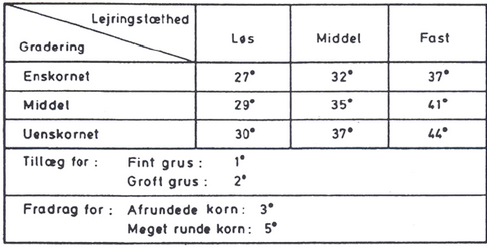
\includegraphics[width=1.2\textwidth]{billeder/friktionsvinkel.png}
		\caption{Friktionsvinkel \citep[ s. 170]{geoteknik}}
		\label{fig:friktionsvinkel}
	\end{minipage}\hfill
\end{figure}

\section{Bæreevne for fundamentet}
Til bestemmelse af bæreevnen af fundamentet benyttes formlen:
\begin{center}
	$\frac{R}{A}=\frac{1}{2}*\gamma*b'*N_\gamma*s_\gamma*i_\gamma+q*N_q*s_q*i_q*d_q+c'*N_c*s_c*i_c*d_c$
\end{center}

Hvor 
$R:effektiv lodret bæreevne
A:effektiv areal 
\gamma:rumvægt for sand - vand som sættes til 20\frac{kN}{m^3}-10\frac{kN}{m^3}
b':effektive bredde
N_\gamma:bæreevnefaktor 
s_\gamma og s_q:formfaktor
i_\gamma og i_q:hældningsfaktor
q:effektiv lodret overlejringstryk ved FUK 
d_q:dybdefaktor$
\newline
\newline
Alle værdier pånær $b'$ kan bestemmes, således $b'$ til sidst kan bestemmes.
I og med der intet moment er i understøtningen, er hele bredden af fundamentet effektiv og dermed ikke excentrisk. Fra resultanten af alle lodrette kræfter i fundamentunderkanten, V, fås en belastning, og for at fundamentet kan holde, skal R mindst være lige så stor som V.
Der beregnes ikke kohæsion, fordi den der næsten ingen kohæsion er imellem sandkornene og dermed betragtes som værende 0. Derfor medregnes $c'*N_c*s_c*i_c*d_c$ -leddet ikke.
Da det ikke altid kan sikres, at jorden ved siden af fundamentet forbliver intakt, ses der normalt bort fra dybdefaktoren, og sættes $d__q$ til 1.
Arealet kan bestemmes, når arealet antages for at være kvadratisk, og da der intet moment er i understøtningen er $b'=b$ og arealet bliver $A=b^2$.

\begin{center}
	$s_\gamma=1-0,\!4*\frac{b'}{l'}=1-0,\!4*\frac{b'}{b'}=1-0,\!4=0,\!6$
	$s_q=1+0,\!2*\frac{b'}{l'}=1+0,\!2*\frac{b'}{b'}=1+0,\!2=1,\!2$
	\newline
	$i_q=(1-\frac{H}{V+A*c'*cot(\varphi)'})^2$
\end{center}

H:resultanten for alle vandrette kræfter i fundamentunderkanten, FUK, som sættes til $1,\!33079214*10^5N$
V:resultanten for alle lodrette kræfter i fundamentunderkanten, FUK, som sættes til $5,\!351696139*10^5N$
\newline
\newline
Da $c'$ ikke anvendes i dette projekt, sættes denne lig 0 og formlen bliver da:
\begin{center}
	$i_q=(1-\frac{H}{V})^2$
	$i_q=(1-\frac{1,\!33079214*10^5N}{5,\!351696139*10^5N})^2=0,\!5645007388$
\end{center}

\begin{center}
	$i_\gamma=i_q^2$
	$i_\gamma=(0,\!5645007388)^2=0,\!3186610841$
\end{center}

$q$ bestemmes, når fundamentet antages at have en højde på 0,8 m(se Figur XX) og der regnes kun for $q__ude$:
\begin{center}
	$q=h_1*\gamma+h_2*(\gamma_sand-\gamma_vand)$
\end{center}

$h_1:$længden ned til grundvandsspejlingen, som er $0,\!8m$
$h_2:$længden fra grundvandsspejlingen ned til fundamentunderkanten, FUK som er $2,\!8m$
$\gamma:$ henholdsvis rumvægten for sand og vand.

\begin{center}
	$q=0,\!8m*20\frac{kN}{m^3}+2m*(20\frac{kN}{m^3}-10\frac{kN}{m^3})=36\frac{kN}{m^2}$
\end{center}

$N_q$ betemmes ud fra følgende formel, når friktionsvinklen,$\varphi=32,\!33$
\begin{center}
	$N_q=e^\pi*Tan(\varphi)*\frac{1+Sin(\varphi)}{1-Sin(\varphi)}$
	$N_q=e^\pi*Tan(32,\!32604742)*\frac{1+Sin(32,\!32604742)}{1-Sin(32,\!32604742)}=24,\!083$
\end{center}

$N_\gamma$ bestemmes ud fra følgende formel: 
\begin{center}
	$N_\gamma=\frac{1}{4}((N_q-1)Cos(\varphi))^\frac{3}{2}$
	$N_\gamma=\frac{1}{4}((24,\!083-1)Cos(32,\!32604742))^\frac{3}{2}=21,\!53664057$
\end{center}

Bredden $b'=b$ kan nu bestemmes: 
\begin{center}
	$\frac{R}{A}=\frac{1}{2}*\gamma*b'*N_\gamma*s_\gamma*i_\gamma+q*N_q*s_q*i_q*d_q$
	$\frac{V}{b^2}=\frac{1}{2}*\gamma*b'*N_\gamma*s_\gamma*i_\gamma+q*N_q*s_q*i_q*d_q$
	$(\frac{5,\!351696139*10^5N}{b^2}=\frac{1}{2}*10000*b*21,\!53664057*0,\!6*0,\!3186610841+36000*24,\!083*1,\!2*0,\!5645007388*1)=0,\!9392506518$
\end{center}
\newline
Dermed skal siderne på fundamentet være 0,94 m.

Efter bredden af fundamentet er bestemt, bør der ses på anvendelses- og brudgrænser, for at sikre mod eventuelle brud. Anvendelsesgrænsen anvendes, når der kigges på stivhedsgraden i jorden. Hvis jordens stivhed ikke er tilstrækkelig, risikerer fundamentet at synke. Det skal sikres, at fundamentet kan sætte sig i jorden, uden at sætte sig for meget, da dette kan resultere i brud af konstruktionen.
\newline \indent{     }  Jorden testes ved at lægge tryk på jorden, og herudfra lave en arbejdskurve, hvor der undersøges hvor sammenpresset jorden er. 
\newline
\newline
Når jord påvirkes af en vertikal kraft, komprimeres jorden lodret, indtil det ikke kan opholdes og derfor skubber ud ad i en spiralform. Brudgrænsetilstanden regnes for at se, om jorden kan holde til belastningen fra bygningen. Dette bestemmes via spiralanalyse, hvor jordtrykket, der vil skubbe med reaktionen, skal være mindre end jordtrykket, som skubber mod reaktionen. Disse kaldes henholdsvis den drivende- og den stabiliserende kraft. Spiralens form afhænger af materialet. For sand er friktionsvinklen afgørende, og for ler er kohæsionen afgørende for vinklen. Ler er mere afrundede spiraler, mens spiralerne for sand er fladere. 
\newline \indent{     }  På Figur XX ses et eksempel for sand, hvilket viser, hvordan scenariet udspiller sig for sandets spiral. For at bestemme både den stabiliserende- og den drivende kraft, opdeles sandet i geometriske områder, og vægten udregnes. På den drivende del bliver fundamentet og dens vægt lagt sammen med vægten af sand. Denne skal også adderes med den vertikale kraft. Den samlede vægt for hele området skal adderes og den stabiliserende kraft skal være større end den drivende kraft. Der laves spiraler rundt om flere punkter, for at sikre at der ikke opstår brud noget sted. 

\section{Delkonklussion}
Aalborgs geologi er analyseret i denne rapport. Jorden i Aalborg består primært af Aalborgler, hvilket der ikke ønskes at arbejde med, da der anvendes pælefundering til ler. I stedet er der valgt at arbejde med boreprofiler fra Hals/Hou, da disse primært består af sand, hvortil der laves direkte fundering, som der ønskes at arbejde med. I et laboratorium er der udført fire forsøg med baskapsand fra Sverige, som antages at være sand fra Hals/Hou området, så disse stemmer overens. Formålet med de fire forsøg er, at finde friktionsvinklen, hvilket er beregnet til 32,33 grader. Der ønskes at lave et punktfundament for hver pæl, som beregnes til at være XX m i både bredden og længden, for at fundamentet har tilstrækkelig bæreevne.